\documentclass[12pt,letterpaper]{article}
\usepackage[utf8]{inputenc}
\usepackage[spanish]{babel}
\usepackage{graphicx}
\usepackage[left=2cm,right=2cm,top=2cm,bottom=2cm]{geometry}
\usepackage{graphicx} % figuras
% \usepackage{subfigure} % subfiguras
\usepackage{float} % para usar [H]
\usepackage{amsmath}
%\usepackage{txfonts}
\usepackage{stackrel} 
\usepackage{multirow}
\usepackage{enumerate} % enumerados
\renewcommand{\labelitemi}{$-$}
\renewcommand{\labelitemii}{$\cdot$}
% \author{}
% \title{Caratula}
\begin{document}

% Fancy Header and Footer
% \usepackage{fancyhdr}
% \pagestyle{fancy}
% \cfoot{}
% \rfoot{\thepage}
%

% \usepackage[hidelinks]{hyperref} % CREA HYPERVINCULOS EN INDICE

% \author{}
\title{Caratula}

\begin{titlepage}
\begin{center}
\large{UNIVERSIDAD PRIVADA DE TACNA}\\
\vspace*{-0.025in}
\begin{figure}[htb]
\begin{center}

\includegraphics[width=8cm]{./Imagenes/logo}
\end{center}
\end{figure}
\vspace*{0.15in}
INGENIERIA DE SISTEMAS  \\

\vspace*{0.5in}
\begin{large}
TITULO:\\
\end{large}

\vspace*{0.1in}
\begin{Large}
\textbf{Informe Laboratorio N° 04} \\
\end{Large}

\vspace*{0.3in}
\begin{Large}
\textbf{CURSO:} \\
\end{Large}

\vspace*{0.1in}
\begin{large}
INTELIGENCIA DE NEGOCIOS\\
\end{large}

\vspace*{0.3in}
\begin{Large}
\textbf{DOCENTE(ING):} \\
\end{Large}

\vspace*{0.1in}
\begin{large}
 Patrick Cuadros Quiroga\\
\end{large}

\vspace*{0.2in}
\vspace*{0.1in}
\begin{large}
Alumna: \\
\begin{flushleft}

Merino Quispe Katerin Almendra  \hfill	(2018060918) \\

\end{flushleft}
\end{large}
\end{center}

\end{titlepage}


%%%%%%%%%%%%%%%%%%%%%%%%%%%%%%%%%%%%%%%%%%%%%%%%%%%%%%%%%%%%%%%%%%%%%%%%%%%
%
% Plantilla para un artículo en LaTeX en español.
%
%%%%%%%%%%%%%%%%%%%%%%%%%%%%%%%%%%%%%%%%%%%%%%%%%%%%%%%%%%%%%%%%%%%%%%%%%%%



%--------------------------------------------------------------------------
\title{Plantilla para un artículo \LaTeX}
\author{El autor va aquí\\
  \small Dept. Plantillas y Editores\\
  \small E12345\\
  \small España
}


\begin{document}
\begin{center}
\textbf{PRACTICA DE LABORATORIO N° 04:} \\
\textbf{Modelamiento Dimensional} \\
\end{center}

\section{REQUERIMIENTOS}

\textbf{- Conocimientos} \\
\textbf{✓ Para el desarrollo de esta práctica se requerirá de los siguientes conocimientos básicos:}
\item{- Conocimientos básicos de administración de base de datos Microsoft SQL Server.\\
- Conocimientos básicos de SQL.\\\\
\textbf{- Software} \\
\textbf{✓ Asimismo se necesita los siguientes aplicativos:} \\
- Microsoft SQL Server 2016 o superior.\\
- Base de datos AdventureWorksDW2016 o superior}

\section{CONSIDERACIONES INICIALES}
\item{Generar todos los modelos fisicos de los diagramas entidad relación y modelo dimensional en bases de datos separadas en Microsoft SQL Server.}

\section{DESARROLLO}
\textbf{Ejercicio N° 01: Envíos} \\
\item{El siguiente diagrama E / R simplificado describe el envío de mercancías. Los lotes pertenecientes a ciertos grupos se envían a ciertos destinos en varios países a través de diferentes modos de transporte. Un cierto centro de costos es responsable de cada envío. La dimensión de tiempo consiste en mes y año.}
\begin{center}
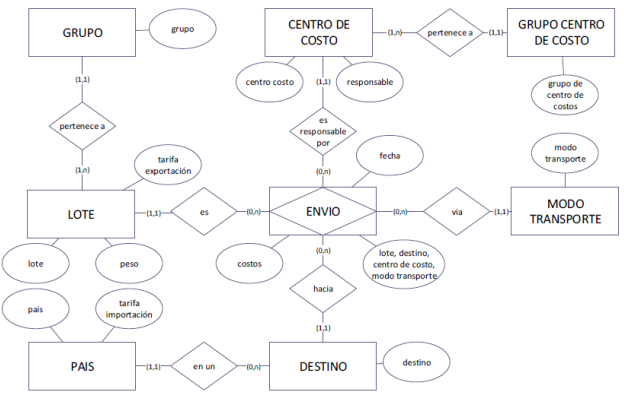
\includegraphics[width=12cm]{./Imagenes/1}
\end{center}

\item{Supongamos que los costos de los atributos ya incluyen todas las tarifas. No se transferirá más información sobre las tarifas al almacén de datos. El análisis tendrá lugar a nivel del grupo de centros de costos, no se necesita información sobre los centros de costos.
Por favor identifique el hecho de interés y construya el Modelo Dimensional y su respectivo diagrama físico}
\begin{center}
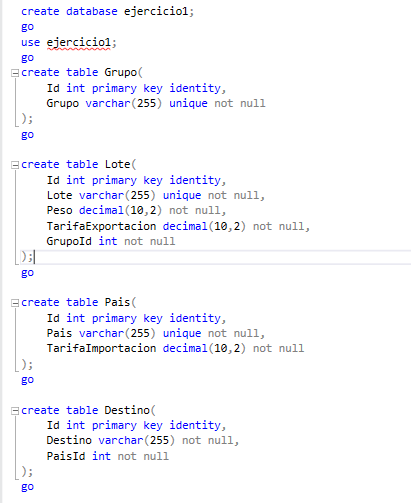
\includegraphics[width=12cm]{./Imagenes/11}
\end{center}

\begin{center}
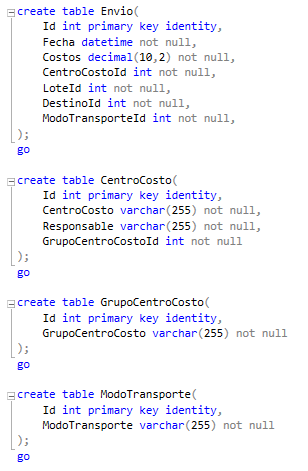
\includegraphics[width=12cm]{./Imagenes/12}
\end{center}
\\
\textbf{Modelo Dimensional}
\begin{center}
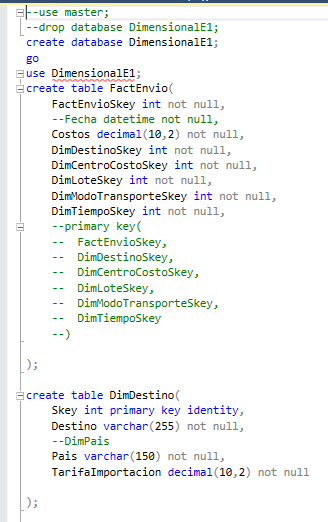
\includegraphics[width=12cm]{./Imagenes/14}
\end{center}

\begin{center}
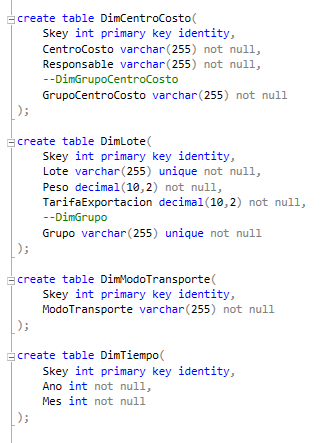
\includegraphics[width=12cm]{./Imagenes/15}
\end{center}

\newpage
\textbf{Ejercicio N° 02: Reservas de viaje}
\item{En este esquema de E / R, un cliente (que es de cierto tipo) reserva un viaje en una agencia de viajes. La agencia de viajes trabaja para un determinado operador turístico. El viaje va a un destino determinado que pertenece a un país determinado.
La dimensión de tiempo consiste en mes, trimestre y año.}

\begin{center}
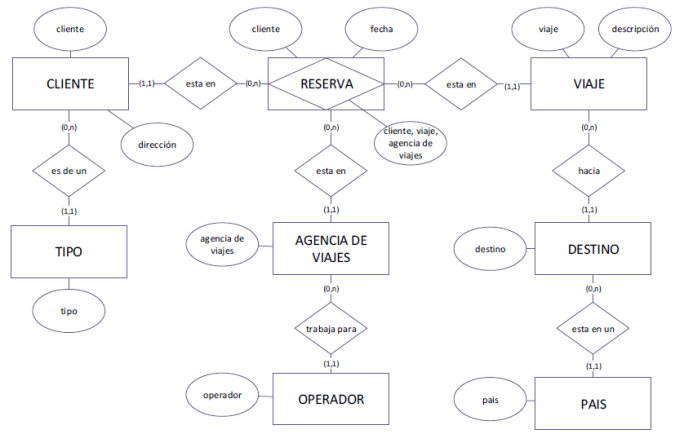
\includegraphics[width=12cm]{./Imagenes/2}
\end{center}
\item{Por favor identifique el hecho de interés y construya el Modelo Dimensional y su respectivo esquema físico}

\begin{center}
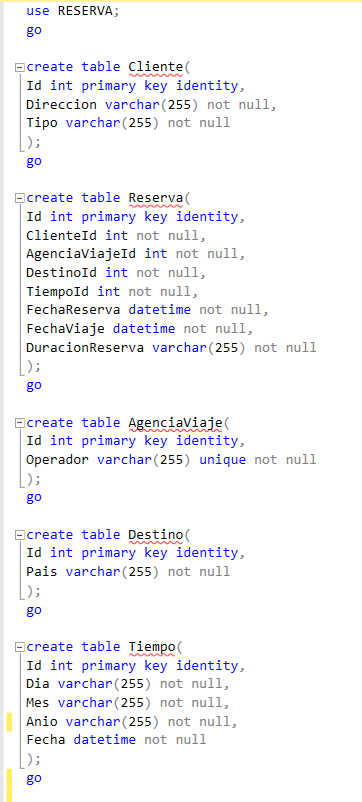
\includegraphics[width=7cm]{./Imagenes/reservacodigo}
\end{center}

\textbf{Modelo Dimensional}
\begin{center}
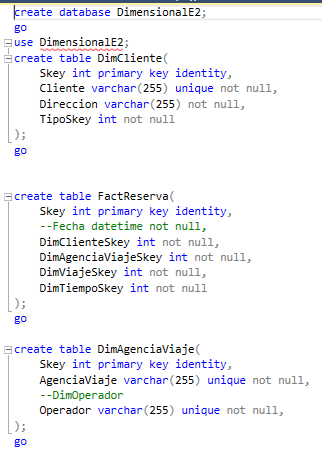
\includegraphics[width=7cm]{./Imagenes/24}
\end{center}
\begin{center}
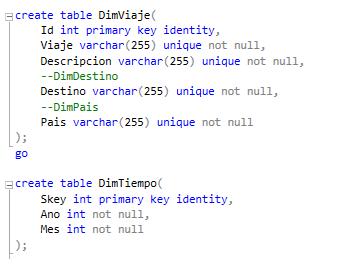
\includegraphics[width=7cm]{./Imagenes/25}
\end{center}


\textbf{Ejercicio N° 03: Gestión de proyectos}
\item{Este esquema E / R simplificado muestra un caso gestión del proyecto.
El proyecto para un cliente se divide en varios paquetes de trabajo y siempre una persona es responsable de completar la tarea. Se cuida en un lugar determinado.
La dimensión de tiempo consiste de día, mes y año.}

\begin{center}
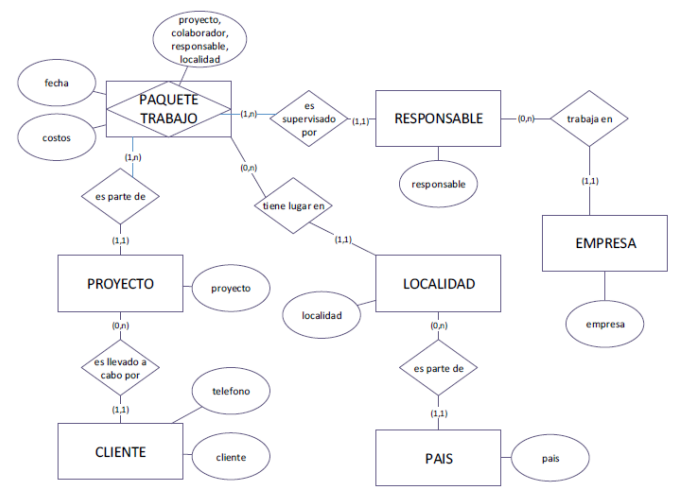
\includegraphics[width=12cm]{./Imagenes/3}
\end{center}
\item{Por favor identifique el hecho de interés y construya el Modelo Dimensional. Incluya un atributo de hecho adicional que cuente la cantidad de paquetes de trabajo. Asimismo, realice el diagrama físico.}

\begin{center}
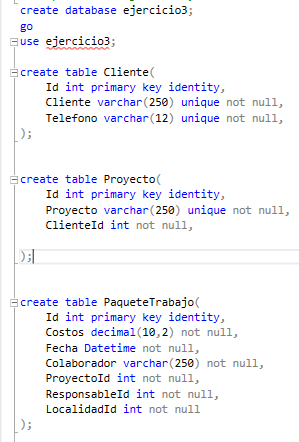
\includegraphics[width=7cm]{./Imagenes/31}
\end{center}

\begin{center}
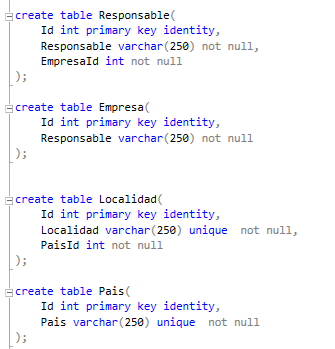
\includegraphics[width=7cm]{./Imagenes/32}
\end{center}
\textbf{}
\textbf{Modelo Dimensional}
\begin{center}
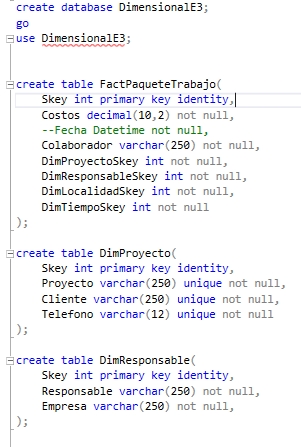
\includegraphics[width=7cm]{./Imagenes/33}
\end{center}

\begin{center}
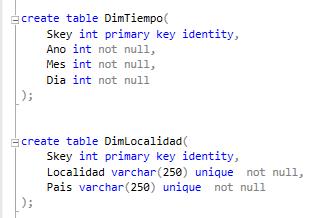
\includegraphics[width=7cm]{./Imagenes/34}
\end{center}

\end{document}


\end{document}
